\documentclass[journal]{IEEEtran}
\usepackage[letterpaper,margin=1.02in,left=1.025in,includefoot,footskip=18pt]{geometry}
\pagestyle{plain}
\setlength{\textfloatsep}{7pt plus 1pt minus 2pt}
\setlength{\dbltextfloatsep}{7pt plus 1pt minus 2pt}
\setlength{\floatsep}{6pt plus 1pt minus 2pt}
\setlength{\dblfloatsep}{6pt plus 1pt minus 2pt}
\renewcommand{\arraystretch}{0.94}
\setlength{\parskip}{0pt plus 0.4pt}
\usepackage{cite}
\usepackage[cmex10]{amsmath}
\interdisplaylinepenalty=2500
\usepackage{amssymb,amsfonts,amsthm}
\usepackage{graphicx,booktabs,multirow,array}
\usepackage{xcolor,url}
\usepackage[hidelinks]{hyperref}
\usepackage{enumitem}
\usepackage[ruled,vlined,linesnumbered]{algorithm2e}
\theoremstyle{definition}
\newtheorem{definition}{Definition}
\theoremstyle{plain}
\newtheorem{proposition}{Proposition}
\newtheorem{theorem}{Theorem}
\hyphenation{post-pro-cess-ing class-i-fi-ca-tion}
\begin{document}
\bstctlcite{IEEEcompactrefs}
\title{Teacher-Health-Guided Release of Differentially Private Speech Classifiers under Class Imbalance}
\author{Yadi Wen, Yaxuan Wang, Dan Yu, Rong Du, Yue Fu, Yongle Chen\\
\IEEEauthorblockA{Shanxi Key Laboratory of Industrial Internet Security, Taiyuan University of Technology, China\\
Emails: \{2023005322, 2023005749\}@link.tyut.edu.cn, \{yudan, durong, fuyue, chenyongle\}@tyut.edu.cn}}
\maketitle
\thispagestyle{plain}

\begin{abstract}
A differentially private speech teacher can be safe to release yet provide unreliable supervision under class imbalance. We study this distinction through Teacher-Conditioned Release Distillation, which chooses exclusion, attenuation, or full use of teacher targets before training the released student. The policy combines class-balanced teacher diagnostics with permitted hard-label learning and distillation; privacy follows separately by post-processing of the accounted teacher. A Common Voice 17.0 study uses 50,000 training clips, ten speaker-grouped partitions, five noise levels, and calibration independent of checkpoint selection. Teacher conditions and student objectives are paired. Across the fixed noise grid, the policy improves mean balanced accuracy by 2.20 percentage points over hard-label training and by 1.29 points over a binary teacher-balanced-accuracy route, without a corresponding improvement in macro-averaged F-measure over hard labels. Component checks distinguish routing gains from predictive value: the composite does not predict distillation gain better than balanced accuracy alone. Likewise, instance-aware attenuation does not outperform a constant, mean-matched reduction of teacher influence. Speaker-cluster uncertainty changes certification and can forgo beneficial supervision. Smaller accent and emotion studies supply low-health and heterogeneous-transfer counterexamples. The results support teacher-conditioned supervision as an explicit release decision while identifying when simple attenuation, direct student validation, or hard-label learning remains competitive.
\end{abstract}
\begin{IEEEkeywords}
Differential privacy, speech classification, model release, knowledge distillation, class imbalance, teacher reliability.
\end{IEEEkeywords}
\IEEEpeerreviewmaketitle

\section{Introduction}
\label{sec:intro}
\IEEEPARstart{S}{peech} classifiers support voice interaction and affective computing~\cite{baltrusaitis2019multimodalSurvey}, but released checkpoints permit inference attacks~\cite{shokri2017membershipInference,fredrikson2015modelInversion}. Differential privacy (DP) bounds individual-record influence~\cite{dwork2006DP,dwork2014}; DP-SGD applies per-example clipping and Gaussian noise~\cite{abadi2016deepLearningDP,mironov2017rdp}. Under imbalance, these operations can weaken minority learning while accuracy conceals majority collapse~\cite{chen2020understandingClipping,tran2021dpimbalance,bagdasaryan2019dpimpact}. A privacy-eligible teacher can consequently provide unreliable student supervision.


We study an audio-only student trained from a private teacher and permitted labeled auxiliary/development speech. \emph{Teacher health} summarizes the class-balanced structure of development predictions. Teacher-Conditioned Release Distillation (TCRD) uses it to exclude, attenuate, or fully use teacher targets before student optimization. Selecting among already trained students uses more direct evidence but requires those candidates; a single teacher-metric threshold is an equally inexpensive alternative. We compare both.



Our earlier work~\cite{wen2026private} studied the private-teacher/offline-student protocol and teacher stabilization. Here we study how teacher supervision enters release:
\begin{itemize}[leftmargin=*,itemsep=2pt]
\item \textbf{Supervision selection:} exclusion, attenuation, and full KD are explicit release actions, distinct from the privacy eligibility of teacher access.
\item \textbf{Routing uncertainty:} confusion-matrix estimation yields health-region probabilities, confidence margins, and a deterministic limit, rather than a student-utility guarantee.
\item \textbf{Paired evidence:} a ten-seed, 50,000-clip CV17 study tests independent calibration, component increment, and mean-matched attenuation; smaller speech studies expose missed beneficial transfer.
\end{itemize}

\begin{figure*}[t]
\centering
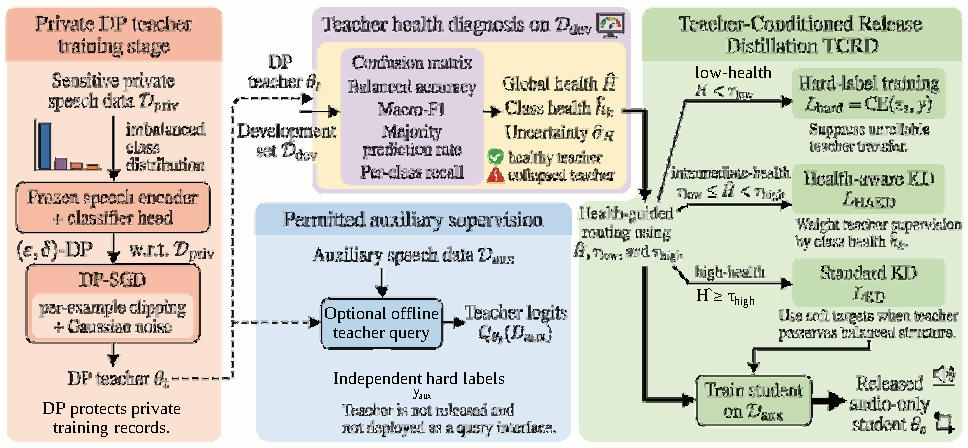
\includegraphics[width=.84\textwidth]{figure/fig1_old_vector.pdf}
\caption{Teacher-health-guided private speech release, illustrated with a frozen-encoder teacher.}
\label{fig:pipeline}
\end{figure*}

\section{Related Work}
\label{sec:related_work}
\subsection{Private Learning and Model Transcription}
DP-SGD with privacy-random-variable (PRV) accounting privatizes training~\cite{abadi2016deepLearningDP,mironov2017rdp,yousefpour2021opacus}; PATE instead privatizes ensemble labels from disjoint private shards~\cite{papernot2017pate,papernot2018pate}. Neither specifies whether a particular teacher should supervise the student.

Model Conversion via Differentially Private Data-Free Distillation~\cite{liu2023datafree} transcribes a teacher using a generator and private gradients; Privacy-Preserving Model Transcription With Differentially Private Synthetic Distillation~\cite{liu2026syntheticdistill} uses noisy supervision in a teacher--student--generator framework. Discriminative--Generative Distillation~\cite{ge2023discriminativegenerative} combines synthetic data, private ensemble labels, and semi-supervised learning. DP-SAD~\cite{liu2024stochasticadversarial} privatizes cross-model diffusion gradients, while Private Gradient Estimation~\cite{liu2024privategradient} perturbs score-estimation projections for generative modeling. TCRD instead selects supervision from an already accounted teacher and permitted labeled speech.


\subsection{Adaptive Distillation and Speech Representations}
Knowledge distillation (KD) transfers structure~\cite{hinton2015distilling}, including in acoustic, representation-compression, and emotion tasks~\cite{chebotar2016distilling,chang2022distilhubert,srinivasan2022representation,shome2024speech}. Difficulty-level KD compares original/pruned teacher predictions~\cite{ham2024difficultykd}; curriculum-temperature KD (CTKD) learns temperature adversarially~\cite{li2023ctkd}. We compare published global-T CTKD with TCRD's teacher-level objective choice, including complete exclusion. Uncertainty-weighted cross-entropy (CE) and linear-temperature KD are separately labeled probes.


Our wav2vec 2.0, HuBERT, and WavLM encoders~\cite{baevski2020wav2vec2,hsu2021hubert,chen2022wavlm} provide contrasting teacher--student conditions. Unlike private acoustic-adapter or ASR-encoder learning~\cite{ho2023differentially,chauhan2024training}, these encoders remain frozen.

\subsection{Class Imbalance and Teacher Health}
Focal loss, class-balanced loss, logit adjustment, and Balanced Softmax (BS) address imbalance~\cite{lin2017focal,cui2019classbalanced,menon2021longtail,ren2020balanced}; private learning can alter class-wise utility~\cite{bagdasaryan2019dpimpact,tran2021dpimbalance,ganev2022robinhood}. We use established BS and test teacher health separately from student transfer.

\section{Problem Formulation and Method}
\label{sec:method}
\subsection{Release Setting and Privacy Boundary}
\label{sec:release_private_learning}
Let $D_{\mathrm{priv}}$ denote private speech and $D_{\mathrm{aux}},D_{\mathrm{dev}}$ permitted labeled auxiliary/development data. An example-level DP mechanism satisfies
\begin{equation}
\Pr[\mathcal M(D)\in S]\le e^\varepsilon\Pr[\mathcal M(D')\in S]+\delta
\label{eq:dp}
\end{equation}
for neighboring private datasets and measurable $S$. Adjacency and sampling follow the accountant; speaker-disjoint splits do not imply speaker-level DP.

Let $Z_t=\mathcal M(D_{\mathrm{priv}})$ include the entire accounted trajectory inspected for development-based checkpoint selection. The release map is
\begin{equation}
\theta_s=\mathcal F(Z_t,D_{\mathrm{aux}},D_{\mathrm{dev}},\nu,\xi),
\label{eq:release_map}
\end{equation}
where $\nu$ is permitted class-prior metadata and $\xi$ private-data-independent randomness. The map includes checkpoint/route selection, health estimation, offline teacher queries, and student training. Auxiliary/development data, labels, and $\nu$ are fixed under adjacency.

\begin{proposition}[Privacy of the adaptive release]
\label{thm:student_privacy}
If $Z_t$ is $(\varepsilon,\delta)$-DP, the complete map~\eqref{eq:release_map}, including the selected route and reported health, is $(\varepsilon,\delta)$-DP for $D_{\mathrm{priv}}$.
\end{proposition}
Standard post-processing proves this (Supplement I-A)~\cite{dwork2014}. A predetermined Hard student is private-data-independent; a teacher-selected Hard route retains the teacher budget. Every inspected private update/candidate must be accounted. Sensitive counts or auxiliary/development records require separate mechanisms and composition, including overlap.


\subsection{Teacher Training and Student Objectives}
\label{sec:teacher_student_objectives}
Teacher/student logits are $z_t=g_{\theta_t}(\phi_t(x))$, $z_s=g_{\theta_s}(\phi_s(x))$, allowing different representations. DP-SGD clips gradients $g_i$ at $C$ and perturbs their sum:
\begin{equation}
\widetilde g=\frac{1}{b_{\mathrm{exp}}}\left[\sum_{i\in\mathcal B}g_i\min\!\left\{1,\frac{C}{\|g_i\|_2}\right\}+\mathcal N(0,\sigma^2C^2I)\right].
\end{equation}
Opacus uses the fixed expected-batch-size normalizer $b_{\mathrm{exp}}$ under Poisson sampling; accounting uses the actual sampling rate, noise, and update count~\cite{abadi2016deepLearningDP,mironov2017rdp}.

For $K$ classes with positive permitted counts $\nu_k$, BS uses~\cite{ren2020balanced}
\begin{equation}
\mathcal L_{\mathrm{BS}}(x,y)=-\log\frac{\nu_y\exp(z_{t,y})}{\sum_{k=1}^K\nu_k\exp(z_{t,k})}.
\label{eq:bs}
\end{equation}
Logit adjustment with $\tau=1$ and priors proportional to $\nu$ is exactly BS~\cite{menon2021longtail}.

For a frozen feature $h$ and linear head, set $p=\operatorname{softmax}(z_t)$, $\bar\nu=\sum_j\nu_jp_j$, and $q_k=\nu_kp_k/\bar\nu$. Then
\begin{equation}
\begin{aligned}
\|\nabla_{w_y}\mathcal L_{\mathrm{CE}}\|_2&=(1-p_y)\|h\|_2,\\
\|\nabla_{w_y}\mathcal L_{\mathrm{BS}}\|_2&=(1-q_y)\|h\|_2.
\end{aligned}
\end{equation}
If $\nu_y<\bar\nu$ and $h\ne0$, BS increases the corrective target-row norm. This pre-clipping identity does not establish post-clipping utility; Supplement I-B derives it.

All student branches use
\begin{equation}
\begin{aligned}
\mathcal L_m(x,y)&=(1-\beta_m(x))\mathrm{CE}(z_s,y)\\
&\quad+\beta_m(x)T^2\mathrm{KL}(p_t^T\Vert p_s^T),
\end{aligned}
\label{eq:unified_student}
\end{equation}
where $p_t^T=\operatorname{softmax}(z_t/T)$, $p_s^T=\operatorname{softmax}(z_s/T)$, and
\begin{equation}
\beta_m(x)=\begin{cases}
0,&m=\mathrm{Hard},\\
\alpha w(x),&m=\mathrm{HAKD},\\
\alpha,&m=\mathrm{KD}.
\end{cases}
\label{eq:action_weights}
\end{equation}
Here $0\le\alpha\le1$, $T>0$; $\beta_m$ excludes, attenuates, or fully retains the KD contribution.

\subsection{Teacher Health and Deterministic TCRD}
\label{sec:tcrd}
For development confusion counts $C_{ij}$ (true $i$, predicted $j$), write row/column totals $C_{k\cdot},C_{\cdot k}$ and $n=\sum_{ij}C_{ij}$. Define
\begin{equation}
\begin{aligned}
\widehat B&=\frac1K\sum_k\frac{C_{kk}}{C_{k\cdot}},&
\widehat F&=\frac1K\sum_k\frac{2C_{kk}}{C_{k\cdot}+C_{\cdot k}},\\
\widehat M&=\max_k\frac{C_{\cdot k}}{n},&
\widehat h_k&=\frac{C_{kk}}{C_{k\cdot}}.
\end{aligned}
\label{eq:metrics}
\end{equation}
These are balanced accuracy, Macro-F1, MajPred, and class recall; zero-denominator terms equal zero. Accuracy is $\sum_kC_{kk}/n$.

The global teacher-health statistic is
\begin{equation}
\widehat H=\lambda_1\widehat B+\lambda_2\widehat F+\lambda_3(1-\widehat M),\quad
\lambda_k\ge0,\quad\sum_{k=1}^3\lambda_k=1.
\label{eq:health}
\end{equation}
The terms measure class coverage, precision--recall balance, and prediction dispersion, respectively. Dispersion alone does not establish correctness.

Weights $\lambda=(1/3,1/3,1/3)$ and thresholds $(\tau_{\mathrm{low}},\tau_{\mathrm{high}})=(0.45,0.60)$ are fixed across tasks/seeds before test evaluation. Sensitivities are reported separately. Dispersion's scale depends on $K$, so these are common conventions, not cross-task calibration.

The deterministic route is
\begin{equation}
m_0(\widehat H)=\begin{cases}
\mathrm{Hard},&\widehat H<\tau_{\mathrm{low}},\\
\mathrm{HAKD},&\tau_{\mathrm{low}}\le\widehat H<\tau_{\mathrm{high}},\\
\mathrm{KD},&\widehat H\ge\tau_{\mathrm{high}}.
\end{cases}
\label{eq:threshold}
\end{equation}
For HAKD,
\begin{equation}
w(x)=\sum_kp_t^T(k\mid x)\widehat h_k,\qquad 0\le w(x)\le1,
\label{eq:hakd_weight}
\end{equation}
Expected class recall is not calibrated correctness. HAKD reduces teacher influence and increases hard-label weight; intermediate weighting need not give intermediate utility.

\paragraph*{What the score can identify}
Health uses hard predictions, whereas KD uses soft targets. Positive logit rescaling preserves $\widehat H$ but changes $p_t^T$ and the KD loss. Student compatibility, auxiliary support, and optimization are also absent from health, so its region need not determine transfer's sign.

\subsection{Uncertainty-Aware Routing}
\label{sec:rctcrd_likelihood}
Health uncertainty is estimated for the selected teacher using permitted calibration data. Earlier runners use 2,000 multinomial draws (audio) or 4,000 (emotion); CV17 additionally resamples speaker clusters on independently held-out calibration data. Supplement I-C derives the fixed-teacher delta-method variance, its regularity conditions, and confidence margins.

Let $G\sim\mathcal N(\widehat H,\widehat\sigma_H^2)$ be a Gaussian working distribution. Extending the three regions in~\eqref{eq:threshold} over the real line gives, for $\widehat\sigma_H>0$,
\begin{equation}
\begin{aligned}
q_{\mathrm{Hard}}&=\Phi(a),\qquad q_{\mathrm{KD}}=1-\Phi(b),\\
q_{\mathrm{HAKD}}&=\Phi(b)-\Phi(a),\\
a&=\frac{\tau_{\mathrm{low}}-\widehat H}{\widehat\sigma_H},\qquad
b=\frac{\tau_{\mathrm{high}}-\widehat H}{\widehat\sigma_H}.
\end{aligned}
\label{eq:routing_masses}
\end{equation}
Here $\Phi$ is the standard-normal CDF. These masses approximate health-region probabilities, not a bounded-support posterior for $H$.

\begin{definition}[Model-conditional region risk]
\label{def:rctcrd-main}
Let $R_G(m)=1-q_m$. RC-TCRD selects the unique mode with $q_m\ge1-\rho$, if one exists, using $\rho=0.10<1/2$. Otherwise it selects Hard with \texttt{certified=false}; fallback is not certification.
\end{definition}
Confidence depends on threshold margin relative to uncertainty. As uncertainty vanishes, the point estimate's region mass tends to one away from thresholds (Supplement Proposition 2). At zero SE, the implementation uses the deterministic route and its tie convention. Sampling from $\operatorname{Categorical}(q)$ is a separate uncertified action; \texttt{zero} refers to routing uncertainty, not KD temperature.

Region disagreement is not negative transfer: $R_G(m)\ne\Pr(\Delta_{\mathrm{KD}}<0)$. The working model provides no distribution-free coverage or student-utility guarantee and does not automatically adjust for same-set selection or speaker dependence.

\begin{algorithm}[t]
\caption{Teacher-conditioned private speech release}
\label{alg:tcrd_release}
\KwIn{$D_{\mathrm{priv}}$; permitted $D_{\mathrm{aux}},D_{\mathrm{dev}},\nu$; training settings; fixed $\lambda,\tau_{\mathrm{low}},\tau_{\mathrm{high}}$; $\kappa\in\{\mathrm{zero},\mathrm{certified},\mathrm{sample}\}$; $\rho=0.10$.}
\KwOut{Released student $\theta_s$ and route record.}
Train the accounted teacher; select its checkpoint on permitted development data\;
Estimate $\widehat H,\widehat h_k$ and uncertainty on the designated calibration data (independent in CV17)\;
\eIf{$\kappa=\mathrm{zero}$}{Set $m=m_0(\widehat H)$\;}{
Compute $q_m$ using the Gaussian working model\;
\eIf{$\kappa=\mathrm{certified}$}{
Select a mode with $q_m\ge1-\rho$ if available; mark certified\;
Else use Hard with \texttt{certified=false}\;
}{Sample $m\sim\operatorname{Categorical}(q)$; mark uncertified\;}}
\If{$m\ne\mathrm{Hard}$}{Cache teacher logits on $D_{\mathrm{aux}}$ offline\;}
Train on $D_{\mathrm{aux}}$ using~\eqref{eq:unified_student}; select on permitted $D_{\mathrm{dev}}$\;
Release the student and record its selected mode\;
\end{algorithm}

\section{Experiments}
\label{sec:experiments}
We first examine low-health and cross-task stress tests; Section~\ref{sec:cv17} then studies larger CV17 data with independent calibration. Protocols are reported separately.

\subsection{Protocol, Metrics, and Comparators}
\label{sec:exp_setup}
\paragraph*{Data and models}
The small Common Voice archive~\cite{ardila2020commonvoice} contains 6,714/1,061/459 train/dev/test clips labeled US, England, or Indian accent.\footnote{\url{https://zenodo.org/records/12588635}; archive metadata specify the Mozilla Public Dataset License 1.0.} Official splits are client/clip-disjoint. Seeds 0--4 reserve $1/4$ of training clients as auxiliary. SSL-BS uses frozen wav2vec2-base features and linear heads, with auxiliary BS counts; Mel-CE uses mel-CNNs. Teachers train eight epochs, batch 128, $C=8$; students train 15, with $\alpha=0.7$, $T=2$. Noise $\sigma=1,1.5,2$ gives seed-wise PRV $\varepsilon=2.7102$--$3.1598$, $1.3270$--$1.5432$, $0.8918$--$1.0328$ at $\delta=10^{-5}$.

VCTK~\cite{veaux2017vctk} uses 720 utterances in four accent classes: 360 private, 120 auxiliary, and 120 each for dev/test. All splits are speaker-disjoint; seeds 0--2 each lack a different auxiliary class. BS mel-CNN teachers train four epochs, students five. Poisson $q=1/6$, 24 updates, $C=8$, $\sigma=1$ give PRV $\varepsilon=6.0829038771$, $\delta=10^{-5}$ (Supplement II-A). Runs use PyTorch 2.11, Opacus 1.6 and RTX 5090 GPUs. The full implementation is public.\footnote{\url{https://github.com/code-experimenter-alt/THG_RoD}}

\paragraph*{Common Voice implementation}
The encoder is \texttt{facebook/wav2vec2-base}, revision \texttt{0b5b8e8}: mono 16-kHz audio, at most 12 seconds, final-layer mean-pooled 768 features. Mel inputs have 40 bins/100 frames, per-frequency normalization and stabilizer $10^{-5}$. AdamW uses learning rate $10^{-3}$, weight decay $10^{-4}$. Maximum dev Macro-F1 selects checkpoints, with earliest ties. Initialization/order seeds are $s+1000003$/$s+1000004$.

\begin{table}[t]
\centering\scriptsize\setlength{\tabcolsep}{3pt}
\caption{Common Voice training settings.}
\label{tab:app_default_hyperparams}
\begin{tabular}{lll}\toprule
Setting & Small archive & CV17\\\midrule
Teacher/student epochs & 8 / 15 & 80 / 80\\
Batch size & 128 & 256\\
AdamW learning rate & $10^{-3}$ & 0.03\\
Weight decay & $10^{-4}$ & $10^{-4}$\\
Clip norm $C$ & 8 & 2\\
Noise $\sigma$ & 1, 1.5, 2 & .5, 1, 2, 4, 8\\
PRV $\delta$ & $10^{-5}$ & $10^{-5}$\\
KD $(\alpha,T)$ & $(0.7,2)$ & $(0.7,2)$\\
SSL sampling / duration & 16 kHz / 12 s & 16 kHz / 12 s\\
SSL feature / classifier & 768 / linear & 768 / linear\\
Mel input (alternative) & $40\times100$ & --\\\bottomrule
\end{tabular}
\end{table}

\paragraph*{Paired evaluation}
We report balanced accuracy (BalAcc), Macro-F1, and diagnostic MajPred. Paired KD gain is
\begin{equation}
\Delta_{\mathrm{KD}}=\mathrm{BalAcc}(s_{\mathrm{KD}})-\mathrm{BalAcc}(s_{\mathrm{Hard}}).
\label{eq:kd_gain}
\end{equation}
Tables~\ref{tab:cv_release_routing}, \ref{tab:cross_dataset_summary}, \ref{tab:cv17_teachers}, and~\ref{tab:cv17_students} use percent scores as mean (SD); CV17 health and $\varepsilon$ remain unscaled. SSL/Mel abbreviate SSL-BS/Mel-CE. Branches share the teacher/cache, student initialization, and auxiliary order. Routes reuse selected checkpoints. Mean $\pm$ sample SD describes seed variation; branch equality is not independent evidence of improvement.

\paragraph*{Two kinds of simple route}
T-BAcc selects Hard below teacher-dev BalAcc 0.45, otherwise KD. S-BAcc/S-MF1/S-MajPred select among trained Hard/KD/HAKD students by dev BalAcc/Macro-F1/minimum MajPred, breaking ties in that order. TCRD chooses the objective before student training. No route uses test utility.

\subsection{Small Common Voice: Diagnosis and Transfer}
\label{sec:cv_main_results}

\begin{table}[t]
\centering
\caption{Small Common Voice teachers ($\sigma=1$; five seeds).}
\label{tab:cv_accent_baseline_dp_loss}
\scriptsize\setlength{\tabcolsep}{3pt}
\begin{tabular}{lccc}
\toprule
Teacher / loss & Acc & BalAcc & MF1\\
\midrule
Non-DP Mel / CE & $.547\pm.032$ & $.341\pm.025$ & $.297\pm.050$\\
Non-DP SSL / CE & $.522\pm.020$ & $.355\pm.020$ & $.323\pm.042$\\
DP SSL / CE & $.516\pm.032$ & $.329\pm.011$ & $.275\pm.013$\\
DP SSL / BS & $.408\pm.192$ & $.347\pm.024$ & $.236\pm.118$\\
\bottomrule
\end{tabular}
\end{table}

\begin{table}[t]
\centering
\caption{Small Common Voice: health and student BalAcc (\%).}
\label{tab:cv_release_routing}
\scriptsize\setlength{\tabcolsep}{2pt}
\begin{tabular}{lcccccc}
\toprule
Teacher & $\sigma$ & Health & Hard & KD & HAKD & CTKD\\
\midrule
SSL & 1.0 & 22.3(7.2) & 34.8(4.1) & 34.3(2.0) & 35.4(3.0) & 34.3(2.8)\\
SSL & 1.5 & 21.7(6.6) & 34.8(4.1) & 34.1(1.2) & 35.4(3.2) & 33.8(1.1)\\
SSL & 2.0 & 22.8(5.3) & 34.8(4.1) & 33.7(2.1) & 35.4(3.9) & 33.3(1.7)\\
\midrule
Mel & 1.0 & 21.2(2.3) & 35.2(3.1) & 32.7(0.8) & 33.4(0.6) & 33.0(0.4)\\
Mel & 1.5 & 20.7(1.8) & 35.2(3.1) & 33.1(0.2) & 32.8(0.4) & 33.3(0.1)\\
Mel & 2.0 & 20.2(1.0) & 35.2(3.1) & 33.2(0.1) & 33.0(0.4) & 32.9(0.9)\\
\bottomrule
\end{tabular}
\end{table}

In Table~\ref{tab:cv_accent_baseline_dp_loss}, BS raises DP teacher BalAcc from 0.329 to 0.347 but lowers Macro-F1 from 0.275 to 0.236 and increases seed variation. Neither BS nor the non-DP controls produces uniformly strong teachers.

Table~\ref{tab:cv_release_routing} gives negative mean KD gain for both families. At $\sigma=1,1.5,2$, SSL gains are $-0.0053\pm0.0291$, $-0.0075\pm0.0388$, $-0.0110\pm0.0277$ (two positive seeds each); Mel gains are $-0.0250\pm0.0314$, $-0.0207\pm0.0305$, $-0.0200\pm0.0304$ (one positive each). Repeated seeds across noise levels are not independent partitions. These near-chance results are low-utility stress tests.

\begin{figure}[t]
\centering
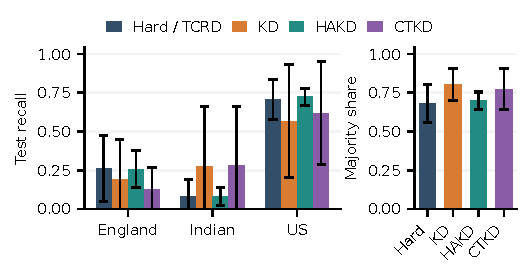
\includegraphics[width=\linewidth]{figure/kd_vs_nokd_seed_only_legend_hatch_two_panels.pdf}
\caption{Small Common Voice SSL-BS: class recall and prediction concentration at $\sigma=1$.}
\label{fig:cv_perclass_kd_diagnostic}
\end{figure}
\begin{figure}[t]
\centering
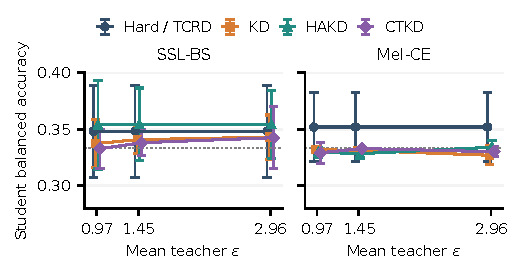
\includegraphics[width=\linewidth]{figure/FIG_stageD_hard_vs_kd_eps_2x2_groupedbars_seed_gradient_nogrid.pdf}
\caption{Small Common Voice privacy sweep (five-seed mean $\pm$ SD).}
\label{fig:cv_privacy_sweep_kd}
\end{figure}

\paragraph*{TCRD versus the simple teacher route}
\label{sec:cv_tcrd_routebalacc}
All health and teacher-dev BalAcc values lie below 0.45. TCRD/T-BAcc choose Hard throughout, and RC certifies Hard. This supplies no composite-score advantage: HAKD has higher SSL mean utility, while Hard leads for Mel. S-BAcc's SSL means are 0.3515/0.3513/0.3542 (Supplement III-C).

Figures~\ref{fig:cv_perclass_kd_diagnostic}--\ref{fig:cv_weak_teacher_tcrd} show the class, privacy, and weak-teacher diagnostics for the same paired seeds. Error bars are sample SDs; dotted lines mark chance. Horizontal offsets in the privacy plot separate methods sharing a budget. Concentrated predictions can accompany lost class-balanced utility.

\begin{figure}[t]
\centering
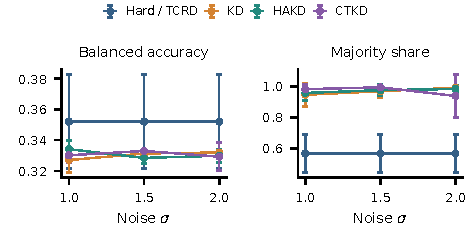
\includegraphics[width=\linewidth]{figure/cv_weak_teacher_tcrd.pdf}
\caption{Weak Mel-CE teachers: paired student utility and prediction concentration.}
\label{fig:cv_weak_teacher_tcrd}
\end{figure}

\begin{table}[t]
\centering\scriptsize\setlength{\tabcolsep}{1.4pt}
\caption{Small Common Voice routing diagnostics.}
\label{tab:app_cv_routing_diagnostics}
\begin{tabular}{llcccc}\toprule
Family & Policy & $\sigma=1$ & $\sigma=1.5$ & $\sigma=2$ & H/A/K\\
 & & \multicolumn{3}{c}{Macro-F1 / MajPred} &\\\midrule
\csname @@input\endcsname{restored_tables/routing_diagnostics.tex}
\bottomrule\end{tabular}
\end{table}
\begin{table}[t]
\centering\scriptsize\setlength{\tabcolsep}{3.3pt}
\caption{SSL-BS privacy sweep and paired KD gains.}
\label{tab:app_cv_privacy_sweep_gain}
\begin{tabular}{rrrrrrr}\toprule
$\sigma$ & $\bar\varepsilon$ & Hard & KD & $\Delta B$ & $\Delta F$ & $\Delta M$\\\midrule
\csname @@input\endcsname{restored_tables/privacy_gain.tex}
\bottomrule\end{tabular}
\end{table}

In Table~\ref{tab:app_cv_routing_diagnostics}, H/A/K count Hard/HAKD/KD decisions. Table~\ref{tab:app_cv_privacy_sweep_gain} gives mean $\varepsilon$, Hard/KD BalAcc, and KD-minus-Hard BalAcc/Macro-F1/MajPred differences in percentage points. Lower MajPred need not imply better classification.

\paragraph*{Additional Mel-BS condition}
Ten separately cached Mel-BS teachers at $\sigma=1,1.5$ give all-negative KD gains, means $-0.0265/-0.0262$; TCRD selects Hard. Supplement III-C specifies this distinct condition.

\subsection{VCTK: Paired Release and Alternative Supervision}
\label{sec:vctk_release}
Table~\ref{tab:vctk_release} includes directly released DP teachers and non-DP CE/BS controls matched on architecture, split, four epochs, optimizer and dev selection. TCRD selects Hard in all three seeds, avoiding negative mean KD gain but rejecting a small positive seed-wise gain. Near-chance utility makes this a limited-support stress test.


\begin{table}[t]
\centering
\caption{Cross-dataset release and VCTK controls (percent scores).}
\label{tab:vctk_release}
\label{tab:cross_dataset_summary}
\scriptsize\setlength{\tabcolsep}{2pt}
\begin{tabular}{llcccc}
\toprule
Dataset & Model & Acc & BalAcc & MF1 & MajPred\\
\midrule
VCTK & Non-DP CE & 22.5(5.1) & 22.5(5.1) & 14.0(2.0) & 70.3(27.3)\\
VCTK & Non-DP BS & 28.6(3.4) & 28.6(3.4) & 17.5(5.2) & 66.9(23.6)\\
\midrule
\csname @@input\endcsname{restored_tables/cross_dataset.tex}
\midrule
VCTK & CTKD, global & 20.6(8.2) & 20.6(8.2) & 13.5(5.7) & 61.9(10.2)\\
VCTK & S-BAcc & 25.3(4.3) & 25.3(4.3) & 16.6(4.9) & 78.3(16.6)\\
VCTK & PATE & 25.6(11.1) & 25.6(11.1) & 16.7(7.6) & 60.8(9.6)\\
VCTK & PATE + labels & 28.9(5.5) & 28.9(5.5) & 17.2(6.6) & 72.5(21.4)\\
\bottomrule
\end{tabular}
\end{table}

\begin{figure}[t]
\centering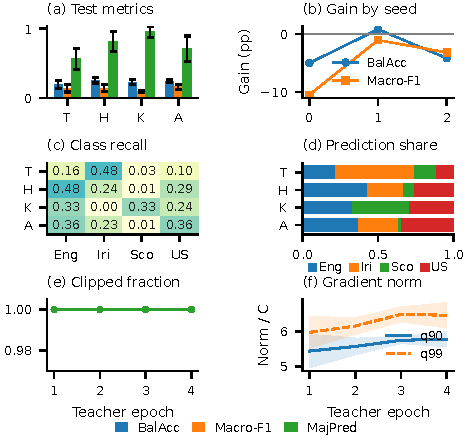
\includegraphics[width=\linewidth]{figure/vctk_main_rich_figure.pdf}
\caption{VCTK paired release and training diagnostics.}
\label{fig:app_vctk_main}
\end{figure}

In the diagnostic figures, T/H/K/A denote teacher/Hard/KD/HAKD. Figure~\ref{fig:app_vctk_main} averages English/Irish/Scottish/US class diagnostics over three seeds. Gains compare paired KD and Hard students; pre-clipping gradient quantiles show mean $\pm$ SD, normalized by $C$. Clipping fraction describes optimization, not routing utility. These public-benchmark gradient diagnostics are not DP release outputs.


Global-T CTKD uses the published temperature and gradient-reversal mechanism under matched training. The two explicit uncertainty/linear-temperature probes are not reproductions (Supplement II-B). PATE matches features, student architecture, initialization/order, five epochs and reported privacy bound. Adding permitted labels raises its mean above Hard/TCRD, with substantial three-seed variation; matching bounds does not equate privacy mechanisms (Supplement II-F).

\paragraph*{HAKD and health components}
Uniform/confidence/class HAKD obtains BalAcc $0.228/0.253/0.244$, versus instance HAKD's 0.239; full SDs and formulas appear in Supplement II-B. This sensitivity does not identify a uniquely optimal weight.

Ten component settings mostly select Hard. Dispersion alone selects HAKD once, lowering mean BalAcc to 0.242. Strict-pair health--gain Pearson/Spearman correlations are $(-0.965,-1.000)$, versus $(0.479,0.500)$ for BalAcc. Three seeds do not establish predictive increment (Supplement II-D).

\subsection{Uncertainty and Threshold Sensitivity}
\label{sec:uncertainty_results}
Development sizes $30/60/120$ cross four fixed threshold pairs. Retraining uses each restricted set throughout selection and calibration: nine teachers, 27 students. Defaults select Hard; near-boundary RC fallback can improve or reduce utility. Supplement II-C reports the full grid and earlier overlapping held-out-health checks, which do not establish population coverage.

\subsection{Other Transfer Conditions and Release Cost}
\label{sec:cross_dataset}
\paragraph*{Fixed-backbone weak teachers}
Five-seed VCTK Mel-CE health spans 0.1278--0.3123. Hard/KD/HAKD BalAcc is $0.2633/0.2733/0.2667$: weak hard predictions can still support useful KD (Supplement II-E).

\paragraph*{Heterogeneous teacher and student}
For frozen HuBERT-to-mel transfer, TCRD chooses Hard (BalAcc 0.2306), below KD (0.2750), CTKD (0.3111) and S-BAcc (0.2722). Supplement II-E reports all paired means/SDs and the replayed privacy budget.

\paragraph*{Emotion classification}
IEMOCAP~\cite{busso2008iemocap} uses open WavLM features.\footnote{\url{https://doi.org/10.5281/zenodo.17803295}, D. Yohanes and A. Chowanda, CC BY 4.0; raw USC audio has separate terms.} Removing unidentified rows and pooling identified variants yields 5,531 utterances, speaker-disjoint across private/aux/dev/test (3,259/1,031/590/651). Five-seed Hard/KD/HAKD BalAcc is $0.478/0.506/0.489$, teacher PRV $\varepsilon=1.840516$, $\delta=10^{-5}$. Both routes select Hard throughout, excluding useful KD (Supplement III-A--B).

\begin{figure}[t]
\centering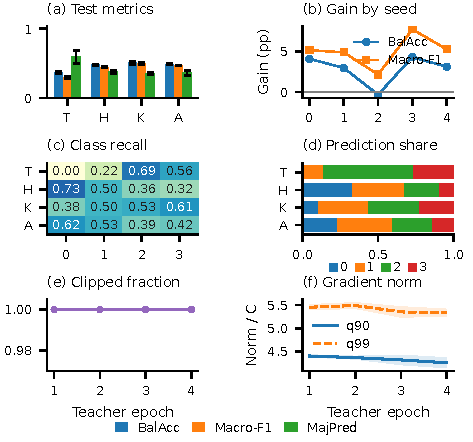
\includegraphics[width=\linewidth]{figure/ieo_iemocap_composite.pdf}
\caption{IEMOCAP paired release and training diagnostics.}
\label{fig:app_iemocap_main}
\end{figure}
\begin{figure}[t]
\centering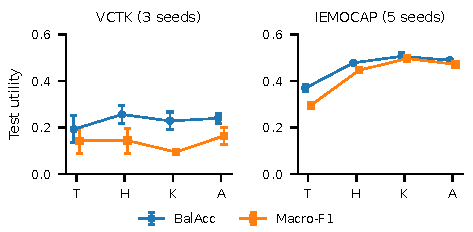
\includegraphics[width=\linewidth]{figure/vctk_iemocap_summary.pdf}
\caption{Cross-dataset teacher and student utility (mean $\pm$ SD).}
\label{fig:vctk_iemocap_summary}
\end{figure}

Figure~\ref{fig:app_iemocap_main} averages five seeds, retains released class IDs 0--3, and shows all four teacher epochs. Figure~\ref{fig:vctk_iemocap_summary} compares methods within each protocol; positive IEMOCAP KD gain contradicts exclusion based solely on low health.

\paragraph*{Release overhead}
The 108 matched warm-cache measurements comprise two small-archive model families, three seeds, three repeats and six policies, with 15 student epochs and CUDA synchronization. TCRD/S-BAcc take $0.218/0.790$~s (SSL), $0.738/2.319$~s (Mel); S-BAcc trains three candidates. Supplement II-F reports every policy, health overhead and memory. These all-Hard-route timings exclude common teacher/feature costs and do not describe CV17's 80 epochs.

\section{CV17 with Independent Calibration}
\label{sec:cv17}
CV17 supplies a higher-utility teacher regime with independent health calibration. Data, optimization, noise, routing, and comparisons were fixed before teacher training/test evaluation. This separate protocol does not reconstruct the earlier manuscript's unavailable partition.

\subsection{Data, Optimization, and Paired Controls}
\label{sec:cv17_protocol}
\paragraph*{Fixed data and speaker separation}
The English CV17 mirror (revision \texttt{8262c16}, CC0-1.0)\footnote{\url{https://huggingface.co/datasets/fsicoli/common_voice_17_0}; pinned third-party mirror.} supplies England/British, Indian/South Asian and US accents (Table~\ref{tab:app_data_stats}). Source-compatible TSV parsing uses \texttt{csv.QUOTE\_NONE}. Of 445,742 eligible rows, shuffling and capping at 20 clips/client (seed 20260908), then sampling (20260909), yields the training corpus.

Class-stratified client splitting of 1,458 development clips (seed 20260910) separates selection and calibration. Client and clip IDs are pairwise disjoint across all four sets; client IDs proxy speakers. Seeds 0--9 reserve $1/4$ of training clients for auxiliary learning, measuring partition/optimization variation on this fixed corpus.

\begin{table}[t]
\centering\scriptsize\setlength{\tabcolsep}{3.4pt}
\caption{CV17 client-disjoint corpus counts.}
\label{tab:app_data_stats}
\begin{tabular}{lrrrrr}\toprule
Split & Clips & England & Indian & US & Clients\\\midrule
\csname @@input\endcsname{restored_tables/data_stats.tex}
\bottomrule\end{tabular}
\end{table}

Seed 0 has 37,462/12,538 private/auxiliary clips, with class counts $(7,228,5,676,24,558)$ and $(2,496,1,554,8,488)$. All seed-wise partitions are saved. Calibration assesses the selected teacher on a different speaker group without consulting test outcomes.

\paragraph*{Features and optimization budget}
The pinned IV-A encoder successfully processes all 53,133 clips: mono 16~kHz, 12-second truncation, real-waveform normalization, fixed zero padding to 12 seconds, and mean pooling over valid final-layer frames. Fixed padding removes batch-composition dependence. Each seed fits an auxiliary-only standardizer, then unit $\ell_2$ normalization. Teacher/student heads are linear $768\to3$.

Teachers/students use 80 epochs, AdamW learning rate 0.03, weight decay $10^{-4}$, and batch 256, following a development-only non-DP check on IV-A's different archive. DP BS uses auxiliary counts, $C=2$, and $\sigma=0.5,1,2,4,8$. Unit features bound the full linear CE/BS gradient (including bias) by 2. Controls are non-DP CE/BS and DP CE at $\sigma=1$. Maximum selection Macro-F1 chooses checkpoints, earliest on ties; calibration never selects.

Private sizes 37,333--37,705 give Poisson $q=1/146,1/147,1/148$ and 11,680--11,840 updates. Opacus 1.6 PRV accounts for all 80 epochs, with tolerances 0.01 in $\varepsilon$ and $\delta/1000$ at $\delta=10^{-5}$. Each bound protects one head-training condition, not encoder pretraining, auxiliary data or a joint release of all teachers. Public-benchmark seeds aid reproduction; private deployment needs undisclosed noise and composition of all inspected runs.

\paragraph*{Attenuation and routing controls}
Each DP BS teacher supplies KD, instance/class/confidence HAKD, global-T CTKD and mean-matched KD students. Hard is shared across noise settings within seed; initialization/order use $s+1000003$/$s+1000004$. KD uses $\alpha=0.7,T=2$; CTKD retains its published mechanism and ten-epoch ramp. Uniform HAKD equals KD at loss/gradient level and reuses its run. There are 80 teachers and 310 students.

Mean-matched KD uses constant KL/CE weights $(\alpha\bar w,1-\alpha\bar w)$, where $\bar w$ averages~\eqref{eq:hakd_weight} over auxiliary examples using the same teacher/calibration recalls. It isolates average attenuation from instance variation. TCRD/RC retain equal weights and $(0.45,0.60)$; binary T-BAcc retains 0.45. Three-way $B$-only routing uses both TCRD thresholds. S-BAcc selects Hard/KD/HAKD on selection BalAcc, ties in that order.

\subsection{Teacher and Student Outcomes}
\label{sec:cv17_outcomes}
\begin{table}[t]
\centering\scriptsize\setlength{\tabcolsep}{2pt}
\caption{CV17 teachers and calibration (ten seeds).}
\label{tab:cv17_teachers}
\begin{tabular}{lcccc}\toprule
Teacher & PRV $\varepsilon$ & BalAcc & MF1 & Health range\\\midrule
\csname @@input\endcsname{cv17_tables/teachers_compact.tex}
\bottomrule\end{tabular}
\end{table}

\begin{table*}[t]
\centering\scriptsize\setlength{\tabcolsep}{3pt}
\caption{CV17 paired students: BalAcc / Macro-F1, in percent (ten seeds).}
\label{tab:cv17_students}
\begin{tabular}{lccccc}\toprule
Mode & $\sigma=0.5$ & $\sigma=1$ & $\sigma=2$ & $\sigma=4$ & $\sigma=8$\\\midrule
\csname @@input\endcsname{cv17_tables/students_compact.tex}
\bottomrule\end{tabular}
\end{table*}

Table~\ref{tab:cv17_teachers} shows non-DP CE/BS BalAcc 0.701/0.729, with lower BS Macro-F1. DP BS/CE at $\sigma=1$ gives BalAcc 0.694/0.665 but Macro-F1 0.653/0.676. BS changes the precision--recall trade-off. Both corpus and optimization differ from IV-A, so this does not isolate data size.

In Table~\ref{tab:cv17_students}, KD-minus-Hard BalAcc gains across increasing $\sigma$ are $+4.47,+3.30,+1.51,-0.63,-4.07$ points, positive in $10/10/8/4/0$ seeds. Health 0.530--0.631 selects 24 KD and 26 HAKD branches, no Hard. The separate low-health studies in IV supply the exclusion cases.

Grid-averaged TCRD-minus-Hard BalAcc is $+2.20$ points (95\% paired seed interval $[1.53,2.81]$); gains over binary/three-way $B$ routes are $+1.29/+0.48$ (Table~\ref{tab:cv17_contrasts}). Macro-F1 versus Hard is $-0.28$ points ($[-0.80,0.24]$). Versus S-BAcc, BalAcc is $-0.21$ ($[-0.41,0.01]$) and Macro-F1 $-0.91$ ($[-1.19,-0.61]$): student validation remains competitive.

\paragraph*{What HAKD contributes}
Instance HAKD beats both Hard and KD in 35/50 conditions, with grid-mean BalAcc gains $+2.43/+1.51$ points. At $\sigma=8$, its mean BalAcc is 0.675 versus Hard's 0.679 and KD's 0.638: attenuation reduces but does not eliminate negative transfer. Versus mean-matched KD it differs by $-0.0016$ points ($[-0.17,0.18]$); Macro-F1 differs by $-0.023$ ($[-0.19,0.14]$). The evidence supports attenuation, not an instance-specific advantage. Class/confidence weights remain competitive.

\subsection{Incremental Value and Uncertainty}
\label{sec:cv17_incremental}
\paragraph*{Prespecified component and gain checks}
Components use equal weights, singles, leave-one-out averages, and permutations of $(0.5,0.25,0.25)$, distinct from VCTK's biased weights. Utilities reuse paired branches; H/A/K counts cover 50 conditions. Grid summaries first average five noises within seed, then summarize ten seeds; 95\% intervals use 20,000 paired seed resamples without multiplicity adjustment. These quantify run variation on fixed cohorts.

Leave-one-seed-out ridge regression (penalty 1) predicts KD-minus-Hard gain from $B$, $H$, or $(B,F,1-M)$. Standardization and fitting use the other nine seeds; held-out errors average each seed's five noises. This checks fixed-corpus prediction, not a test-trained policy.

Table~\ref{tab:cv17_components} shows changed routes without indispensable components: dispersion-only and leave-$B$-out always select HAKD, BalAcc 0.703 versus equal weights' 0.701. Health--gain Pearson/Spearman correlations are 0.858/0.857, versus $B$'s 0.872/0.881 (Fig.~\ref{fig:cv17_gain}). Useful routing and incremental gain prediction are distinct.

Held-out MSEs for $B/H$/all components are $3.06/3.35/3.47\times10^{-4}$. Composite-minus-$B$ MSE is $0.29\times10^{-4}$ (95\% seed interval $[-0.47,1.00]\times10^{-4}$); all-components-minus-$B$ is $0.41\times10^{-4}$ ($[0.012,0.95]\times10^{-4}$). Richer scores do not improve prediction; TCRD's routing gain concerns the specified score/threshold choices.

\begin{table}[t]
\centering\footnotesize\setlength{\tabcolsep}{3pt}
\caption{CV17 health-component ablations (ten seeds).}
\label{tab:cv17_components}
\begin{tabular}{lccc}\toprule
Weighting & H/A/K & BalAcc & Macro-F1\\\midrule
\csname @@input\endcsname{cv17_tables/components.tex}
\bottomrule\end{tabular}
\end{table}

\begin{table}[t]
\centering\footnotesize\setlength{\tabcolsep}{4pt}
\caption{CV17 paired BalAcc differences (percentage points; 95\% seed intervals).}
\label{tab:cv17_contrasts}
\begin{tabular}{lrc}\toprule
Comparison & Mean & Bootstrap 95\% interval\\\midrule
\csname @@input\endcsname{cv17_tables/contrasts.tex}
\bottomrule\end{tabular}
\end{table}

\begin{figure}[t]
\centering
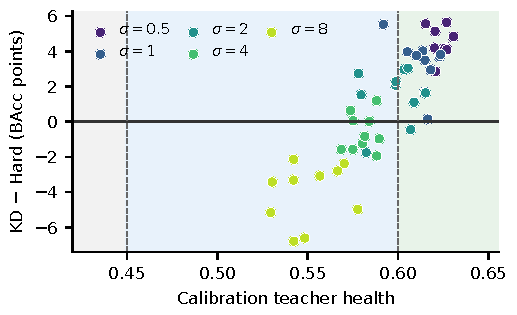
\includegraphics[width=\linewidth]{figure/cv17_health_gain.pdf}
\caption{CV17 calibration health versus paired KD gain.}
\label{fig:cv17_gain}
\label{fig:cv_health_vs_gain}
\end{figure}

\paragraph*{Independent calibration and speaker dependence}
For each selected teacher, 2,000 calibration-speaker bootstrap draws retain every utterance within sampled clusters. Their health SD enters the same Gaussian region rule; multinomial SE is the comparator. Test health is report-only, a noisy finite held-out proxy, not a population-coverage target.

Mean cluster SEs span 0.0185--0.0195 versus multinomial 0.0142--0.0148, changing 12/50 RC decisions. Cluster RC certifies 16 and falls back in 34, reducing BalAcc versus TCRD by 1.70 points ($[-2.16,-1.25]$); Macro-F1 changes $+0.10$ ($[-0.32,0.51]$). Deterministic/RC actions disagree with test-health regions in 15/36 cases; only two RC disagreements are certified. Nominal 95\% cluster intervals contain test-health points in 37/50 cases. Independent calibration removes same-set selection, not the distinction between region confidence and useful transfer.


\section{Conclusion}
\label{sec:conclusion}
TCRD makes exclusion, attenuation, or full KD an explicit private-release decision. CV17 shows balanced-accuracy gains over Hard and fixed BAcc routes; smaller studies expose missed beneficial transfer. BAcc predicts gain at least as well, mean-matched attenuation matches instance HAKD, and student validation remains competitive. Independent calibration and cluster resampling reveal certification's utility cost. Privacy, region confidence, and student utility are distinct properties.
\bibliographystyle{IEEEtran}
\bibliography{bibtex/bib/IEEEabrv}
\end{document}
